%********************************************************************************************
%								COMANDOS ÚTILES PARA LATEX EN ESTE TP							
%
%	\ : espacio simple
%	\\ : nueva línea
%	\par : va a la línea de abajo y deja sangría
%	\vspace{##tamaño en pt##} o \vspace{\baselineskip} en general:
%								 para dejar un espacio vertical
%	\textbf{text} :text en negrita
%	\textit{text} :text en itálica
%
% GRAFICOS CENTRADOS:
%	\begin{center}
%		\includegraphics[width=\textwidth]{./img/##ruta imagen (no hace falta extension)##}
%	\end{center}
%		--> se pueden agregar atributos como scale por si se hace muy grande
%
% TABLAS CENTRADAS:
%	\begin{center}
%	\begin{tabular}{|c|c|}
%	\hline
%	\ \textbf{Programa} & \textbf{Ticks} \\
%	\hline
%		ASM & 675127609 \\
%	\hline
%	\end{tabular}
%	\end{center}
%
% ALGORITMOS (EN VARIOS LENGUAJES):
% \begin{lstlisting}
%	void sumoDiez(int &num)
%	{
%	    num += 10;
%	}
%	
%	int main()
%	{
% 	   int i;
%	    int numeroAProcesar = 20;
%	    for (i = 0; i < 50; i++)
%	    {
%	        sumoDiez(numeroAProcesar);	//Proceso el numero en cada ciclo
%	    } 
%	    return 0;
%	}
%	\end{lstlisting}
%
% para info sobre todo lo que tiene el package detallado:
% http://en.wikibooks.org/wiki/LaTeX/Source\_Code\_Listings
%
%********************************************************************************************

\documentclass[10pt,a4paper]{article}
\usepackage[utf8]{inputenc} % para poder usar tildes en archivos UTF-8
\usepackage[spanish]{babel} % para que comandos como \today den el resultado en castellano
\usepackage{a4wide} % márgenes un poco más anchos que lo usual
\usepackage[conEntregas]{caratula}
\usepackage{amssymb}
\usepackage{fancybox}
\usepackage[usenames,dvipsnames]{color}
\usepackage{hyperref}
\usepackage{listings}
\usepackage{clrscode3e}
\usepackage{xcolor}
\usepackage{amsmath}


\hypersetup{
    colorlinks,
    citecolor=black,
    filecolor=black,
    linkcolor=black,
    urlcolor=black
}

\lstdefinestyle{customc}{
  belowcaptionskip=1\baselineskip,
  breaklines=true,
  frame=L,
  xleftmargin=\parindent,
  language=C,
  showstringspaces=false,
  basicstyle=\footnotesize\ttfamily,
  keywordstyle=\bfseries\color{green!40!black},
  commentstyle=\itshape\color{purple!40!black},
  identifierstyle=\color{blue},
  stringstyle=\color{orange},
}

\lstset{escapechar=@,style=customc}

\begin{document}

\titulo{Trabajo Práctico 1}
\subtitulo{Monkey Island [Primera entrega]}

\fecha{\today}

\materia{Métodos Numéricos}
\grupo{Grupo Autodenominado "Los Pichis"}

\integrante{De Sousa Bispo, Germán Edgardo}{359/12}{german\_nba11@hotmail.com}
\integrante{De Sousa Bispo, Mariano Edgardo}{389/08}{marian\_sabianaa@hotmail.com}
\integrante{Valdés Castro, Tobías}{800/12}{tobias.vc@hotmail.com}


\maketitle

\tableofcontents
\newpage

\section*{Introducción}
\addcontentsline{toc}{section}{Introducción}

El problema que se nos presentó es el del capitán Guybrush Threepwood (un gran pirata) y su barco ``El Pepino Marino''. La existencia de las raras sanguijuelas mutantes ocasiona malestar a nuestro estimado capitán. Las mismas se adhieren al parabrisas de la nave y generan temperatura que pone en peligro la integridad del mismo. La transmisión del calor por parte de las sanguijuelas se produce de manera circular y la temperatura es idéntica para todas ellas. 
\par 
El parabrisas no es invencible: si la temperatura en su punto central supera los 235 grados centígrados, las sanguijuelas ganan y el parabrisas se rompe, dejando al capitán Guybrush Threepwood a la merced de las alimañas mutantes. A este punto central se lo denominará \textit{punto crítico}.
\par 
Sin embargo, el parabrisas posee un mecanismo de defensa ante las criaturas. Los bordes emiten temperaturas bajo cero, para permitir el enfriamiento y así vencer a las sanguijuelas. El sistema de refrigeramiento emite -100$^{o}$C en todo el borde del parabrisas, disminuyendo de esta forma la temperatura global de la superficie. 
\par 
A su vez, nuestro querido capitán Threepwood posee un pollo de hule (el arma más temible para las criaturas de los Siete Mares) con el cual puede destruir sanguijuelas. Sin embargo, el uso del ``Gran Pollo'' es agotador para Guybrush, por lo que debe intentar utilizarlo la menor cantidad de veces posibles para no comprometer el resultado de la misión. 

\vspace{\baselineskip}
\par 
Es nuestro deber, como aspirantes a piratas (informáticos), ayudar al capitán Threepwood para determinar la temperatura en el punto crítico y saber si es necesario utilizar el pollo de hule para matar a las malvadas sanguijuelas. Para ello, llevamos la situación al mundo de la Computación: ya que no podemos representar los infinitos puntos que forman el parabrisas, utilizaremos una discretización que nos permitirá computar la resolución a este problema. 
\par
Gracias a las fórmulas otorgadas por la cátedra para obtener la temperatura en cada punto del parabrisas, calcularla en el punto crítico implica saber además \textit{la temperatura en todos los otros puntos}. Es por esto que encontrar una solución al problema se traduce a \textit{plantear y resolver un sistema lineal en el que las incógnitas son las temperaturas de cada posición discreta del parabrisas}. Es decir, matemáticamente, queremos encontrar una solución a la ecuación

\[ Ax = b \]

donde $x$ representa el vector con todas las temperaturas punto a punto del parabrisas discretizado. Esto nos obliga entonces a pensar qué son la matriz $A$ y el vector $b$ en esta ecuación, lo cual será explicado en la sección \textbf{Desarrollo}. Para resolver este sistema se deberá utilizar la técnica de \textbf{\textit{Eliminación Gaussiana}} a fin de obtener una matriz triangular superior. Luego, se aplicará un algoritmo de resolución llamado \textbf{\textit{backward substitution}} que se encargará de devolvernos todas las temperaturas de los puntos que hayamos podido discretizar, pudiendo así completar la misión del capitán.

\section{Desarrollo}

\subsection{Ideas y pseudocódigo}

\subsubsection{Pseudocódigo y características generales del problema}

Para comenzar a resolver este problema nos toca pensar un pseudocódigo muy simple que nos sirva de boceto general del problema; crear las matrices, resolver el sistema que queda y ubicar la información donde corresponda:

\vspace{\baselineskip}
\begin{codebox}
\Procname{$\proc{SavingPirateGuybrush}()$}
\li createAllMatricesAndVectors()
\li resolveLinearSystemEquations()
\li putNewInformationInWindshieldMatrix();
\End
\end{codebox} 
\vspace{\baselineskip}
\par

Podemos extender un poco este pseudocódigo, sabiendo que debemos crear la matriz del parabrisas, la matriz $A$ y el vector $b$ y la resolución del sistema que quede se realiza con \textit{eliminación gaussiana} y \textit{backward substitution}:

\vspace{\baselineskip}
\begin{codebox}
\Procname{$\proc{SavingPirateGuybrush}()$}
\li matrix \id{pb\_matrix} = createPBMatrix()
\li matrix \id A = createMatrixA()
\li vector \id b = createVectorB()
\li matrix \id C = gaussianElimination(\id A, \id B)
\li vector \id{resolvedX} = resolveUpperTriangularMatrix(C)
\li recreatePBMatrix(\id{pb\_matrix});
\End
\end{codebox} 
\vspace{\baselineskip}

Asumimos aquí que en cada una de esas funciones tenemos acceso a los parámetros del problema para tener una lectura más simple del pseudicódigo. Básicamente, se crean las matrices y vectores necesarios definiendo sus dimensiones, agregando información de bordes, sanguijuelas, etc., y se resuelve el sistema triangulando con $gaussianElimination(A,B)$ (utiliza una matriz aumentada $A|B$) y con $resolveUpperTriangluarMatrix(C)$ la cual aplica \textit{backward substitution}. Luego se reconstruye la matriz del parabrisas. Pasemos ahora a detallar un poco las ideas para saber qué es $A$ y qué es $b$.

\vspace{\baselineskip}

Como vimos en la introducción, resolver este problema es resolver el problema de $Ax = b$ siendo $x$ las temperaturas en todos los puntos que se hayan podido discretizar del parabrisas. Este vector $x$ tendrá un tamaño de $(n+1) \times (m+1)$ siendo $n+1$ la cantidad de filas de esa matriz y $m+1$ la cantidad de columnas. Estos $n$ y $m$ se despejan de las ecuaciones $a = m \times h$ y $b = n \times h$, es decir, $m = \frac{a}{h}$ y $n = \frac{b}{h}$ donde $a$ es el ancho del parabrisas, $b$ el alto, y $h$ siendo la discretización elegida. 

Veremos ahora qué fue lo que pensamos para determinar $b$, y luego en dos secciones distantas explicaremos las ideas atrás de las dos posibles implementaciones de la matriz $A$. Igualmente para $A$ en ambas implementaciones, queremos que $Ax = b$ sea una multiplicación realizable, luego en principio necesitamos una matriz de alto $(n+1) \times (m+1)$  (el mismo que $x$) ya que si no \textit{no podríamos hacer la multiplicación $Ax$}.

\vspace{\baselineskip}

\vspace{\baselineskip}

{\large \textbf{ $\rhd$ Vector $b$:}}

\vspace{\baselineskip}

 Teniendo en cuenta la siguiente fórmula para el cálculo de temperaturas

\[
\frac{\partial^2T(x,y)}{\partial x^{2}}+\frac{\partial^2 T(x,y)}{\partial y^{2}} \ \cong \ \frac{ t_{i-1,j} + t_{i+1,j} - 4t_{i,j} + t_{i,j-1} + t_{i,j+1}}{h^2} = 0,
\]

que los puntos de los bordes tienen temperatura fija -100${}^o$C y que los puntos afectados por el radio de ataque de las sanguijuelas valen otra temperatura fijada $t_{sang}$ en los parámetros del problema, podemos plantear a $b$ como el vector que sigue esta función partida para cada posición ($i,j$) de la matriz discreta del parabrisas:

$$f_{b}(i,j) = \left\{
\begin{array}{c l}
 -100 & si \ la \ posicion  \ p_{i,j} \ es  \ un \ borde  \ del \ parabrisas\\
 t_{sang} & si \ la \ posicion  \ p_{i,j} \ es \ afectada \ por \ una \ sanguijuela \\
 0 & en \ otro \ caso \ en \ el \ cual \ no \ conozca \ la \ temperatura \ en \ p_{i,j}
\end{array}
\right.
$$

De esta forma, el vector $b$ tendrá un tamaño igual a la cantidad de elementos de la matriz que representa al parabrisas, es decir $(n+1) \times (m+1)$, al igual que el vector $x$.

\subsubsection{Ideas para la implementación con matriz A cuadrada}

Nos queda definir entonces qué es la matriz $A$. Decidimos entonces tener una matriz cuadrada de  $((n+1) \times (m+1)) \times  ((n+1) \times (m+1))$ en la cual cada fila representa un elemento de la matriz discreta del parabrisas. Por ejemplo, la primera fila representaría al elemento (0,0), la segunda al (0,1), la tercera al (0,2), hasta la última que representa al elemento ($n-1,n-1$). A su vez, hay una misma cantidad de columnas para poder multiplicar esta matriz por $x$.

La idea atrás de esto es que, al hacer $Ax$, tengamos \textbf{un sistema de ecuaciones que incluya la derivada parcial simplificada} (que aparecía cuando no se conoce la temperatura de un punto en particular) e igualdades directas como la temperatura en los bordes o en un punto afectado. Para lograr esto, esta matriz se va a componer principalmente de \textit{ceros y unos}.

\vspace{\baselineskip}

Este sería un ejemplo de lo que queremos llevar a cabo: si en la primera fila pongo el primer elemento en 1 y el resto en 0, al multiplicar por el vector de temperaturas-incógnitas estaría teniendo en mi ecuación el valor de $x_1$. Como particularmente la primera posición de la matriz representa a un borde, en $b$ tendría según la función ya presentada un -100 indicando la temperatura fija adecuada. Luego mi ecuación sería $x_1 = -100$, y esto es justo lo que queremos. Para la siguiente temperatura me ubicaria en la segunda fila, y como esta también representa a un borde, debería colocar un $1$ en la segunda posición de la fila, así al multiplicar obtendría el $x_2 = -100$. Luego, para cada fila, voy a mirar el elemento que pertenece a la diagonal de la matriz cuadrada ya que allí se encontrará la temperatura a calcular asociada a esa posición en $x$.

En un caso más complicado como en el de temperatura desconocida, deberíamos poner $1$ en cada lugar correspondiente a $t_{i-1,j}$, $t_{i+1,j}$, $t_{i,j-1}$ y $t_{i,j+1}$ involucrado en la ecuación de la derivada segunda simplificada, y un -4 en $t_{i,j}$. Para que esos valores de $x$ aparezcan en la ecuación, ubicamos los valores en la fila de la matriz A de la siguiente forma: para $t_{i,j}$ simplemente tomo la posición ($i,i$) y coloco allí un -4 (ya que ese es su coeficiente asignado en la ecuación de la derivada parcial simplificada). Para $t_{i,j-1}$ y $t_{i,j+1}$, como solo se cambia una columna, estarán una posición menos o más en $x$, por lo tanto debo poner un 1 a ambos costados del -4. Luego, los siguientes 1 estarán a $(n+1)$ (para tener $t_{i-1,j}$) o $-(n+1)$ (para tener $t_{i+1,j}$) espacios a los costados del -4, ya que $n+1$ es el ancho de la matriz del parabrisas discreto, y al cambiar una fila en la matriz discreta del parabrisas, voy a correrme exactamente $n+1$ espacios para la izquierda o la derecha en la fila de la matriz A.

\vspace{\baselineskip}

\vspace{\baselineskip}

{\large \textbf{ $\rhd$ Un posible ejemplo para este problema:}}

\vspace{\baselineskip}

Veamos un ejemplo para una matriz pequeña como un parabrisas de $2 \times 2$ con discretización 1, sin sanguijuelas. Como habíamos dicho, la matriz discretizada del parabrisas será de tamaño $(n+1) \times (m+1)$, luego de $3 \times 3$ en este ejemplo. Así sería la matriz discreta del parabrisas, la cual llamamos $pb\_matrix$: 

\vspace{\baselineskip}

\[ pb\_matrix = \left( \begin{array}{ccc}
-100 & -100 & -100 \\
-100 & ??? & -100 \\
-100 & -100 & -100 
\end{array} \right)\] 

\vspace{\baselineskip}

Como los primeros y últimos 4 elementos de la matriz discreta del parabrisas son bordes, hay temperatura -100. En el medio desconocemos la temperatura.

Por otro lado, nuestra matriz $A$ tendrá dimensiones cuadradas de $((n+1) \times (m+1)) \times  ((n+1) \times (m+1))$, luego en este caso, será de $9 \times 9$.

\vspace{\baselineskip}

\[A = \left( \begin{array}{ccccccccc}
1 & 0 & 0 & 0 & 0 & 0 & 0 & 0 & 0 \\
0 & 1 & 0 & 0 & 0 & 0 & 0 & 0 & 0 \\
0 & 0 & 1 & 0 & 0 & 0 & 0 & 0 & 0 \\ 
0 & 0 & 0 & 1 & 0 & 0 & 0 & 0 & 0 \\
0 & 1 & 0 & 1 & -4 & 1 & 0 & 1 & 0 \\
0 & 0 & 0 & 0 & 0 & 1 & 0 & 0 & 0 \\ 
0 & 0 & 0 & 0 & 0 & 0 & 1 & 0 & 0 \\
0 & 0 & 0 & 0 & 0 & 0 & 0 & 1 & 0 \\
0 & 0 & 0 & 0 & 0 & 0 & 0 & 0 & 1
\end{array} \right)\] 

\vspace{\baselineskip}

Tal como habíamos dicho, cada fila $i$ de esta matriz representa al elemento $i$ de la matriz del parabrisas (vista como un vector aplanado por filas). En la matriz del parabrisas, los elementos que pudimos completar con -100 representan a los bordes del parabrisas. Siguiendo la descripción que habíamos hecho de la matriz $A$, habrá un 1 en la posición $(i,i)$ para las filas que se correspondan con estos bordes, y el resto de las posiciones serán 0. Esto vale para toda la matriz salvo por el medio, en donde desconocemos la temperatura. Luego para la fila $4$ (empezando a contar desde 0), es decir la fila correspondiente al elemento del medio de la matriz del parabrisas, debemos llenar los casilleros con -4 y 1 según nos convenga para obtener luego de hacer $Ax$ la ecuación de la derivada parcial simplificada.

Los vectores $x$ y $b$ entonces tiene la forma siguiente:

\[ x =  \left( \begin{array}{c}
t_{0,0} \\
t_{0,1} \\
t_{0,2} \\
t_{1,0} \\
t_{1,1} \\
t_{1,2} \\
t_{2,0} \\
t_{2,1} \\
t_{2,2} \\
\end{array} \right), \  b = \left( \begin{array}{c}
-100 \\
-100 \\
-100 \\
-100 \\
0 \\
-100 \\
-100 \\
-100 \\
-100 \\
\end{array} \right)
\] 

Juntando todo nos queda entonces:

\[ Ax = b \]

$$
\left( \begin{array}{ccccccccc}
1 & 0 & 0 & 0 & 0 & 0 & 0 & 0 & 0 \\
0 & 1 & 0 & 0 & 0 & 0 & 0 & 0 & 0 \\
0 & 0 & 1 & 0 & 0 & 0 & 0 & 0 & 0 \\ 
0 & 0 & 0 & 1 & 0 & 0 & 0 & 0 & 0 \\
0 & 1 & 0 & 1 & -4 & 1 & 0 & 1 & 0 \\
0 & 0 & 0 & 0 & 0 & 1 & 0 & 0 & 0 \\ 
0 & 0 & 0 & 0 & 0 & 0 & 1 & 0 & 0 \\
0 & 0 & 0 & 0 & 0 & 0 & 0 & 1 & 0 \\
0 & 0 & 0 & 0 & 0 & 0 & 0 & 0 & 1
\end{array} \right)	\left( \begin{array}{c}
t_{0,0} \\
t_{0,1} \\
t_{0,2} \\
t_{1,0} \\
t_{1,1} \\
t_{1,2} \\
t_{2,0} \\
t_{2,1} \\
t_{2,2} \\
\end{array} \right) = \left( \begin{array}{c}
-100 \\
-100 \\
-100 \\
-100 \\
0 \\
-100 \\
-100 \\
-100 \\
-100 \\
\end{array} \right)
$$
\par
Dejando la matriz aumentada siguiente, a la cual luego le aplicaremos la técnica de \textit{eliminación gaussiana} para triangularla y después resolverla mediante \textit{backward substitution}:
\vspace{\baselineskip}
$$
\left( \begin{array}{c | r}
t_{0,0} & -100\\
t_{0,1} & -100\\
t_{0,2} & -100 \\
t_{1,0} & -100\\
t_{0,1} + t_{1,0} - 4t_{1,1} + t_{1,2} + t_{2,1} & 0\\
t_{1,2} & -100\\
t_{2,0} & -100\\
t_{2,1} & -100\\
t_{2,2} & -100\\
\end{array} \right)
$$

\vspace{\baselineskip}

Después de resolver este sistema, vamos a llenar la $pb\_matrix$ antes mencionada con los nuevos valores calculados y eso es todo.

\vspace{\baselineskip}

\vspace{\baselineskip}
\par
Veremos qué sucede ahora con la implementación la matriz A banda, discutiremos las ideas principales y haremos un enfoque mucho más detallista en la parte de implementación.

\subsubsection{Ideas para la implementación con matriz A banda}

Antes que nada, la implementación con matriz banda se puede realizar por la naturaleza de la matriz A en el otro caso: al tener siempre unos en la diagonal y también algunos unos a $n+1$ espacios del centro (y todo el resto es 0), se nos forma una banda diagonal que podemos extraer de la matriz y trabajar únicamente con eso. En realidad, trabajar con todos los valores de la matriz $A$ cuadrada es ineficiente ya que la gran mayoría de los valores son 0 y por ejemplo todas las iteraciones de la \textit{eliminación gaussiana} que no tengan que ver con la banda \textit{no van a realizar ningún cambio en la matriz porque en esos lugares la matriz ya está triangulada} (son todos ceros).

Ya que el pseudocódigo presentado se mantiene incluso para esta implementación, veremos únicamente los cambios a las principales funciones y en la estructura de la matriz $A$ para que esta forma de enfrentar el problema se realice adecuadamente.

\vspace{\baselineskip}

Como ya dijimos, para esta implementación nos alcanza con tomar la banda de la matriz $A$ cuadrada. La banda tiene un tamaño de $2n+1$ elementos (desde la mitad hay $n$ elementos hacia ambos costados y además cuento aquel de la mitad), por lo cual la matriz $A$ modificada tendrá un tamaño de $(n+1) \times (m+1)$ filas por $2n+1$ columnas, lo cual \textit{a priori} sugiere mucho menos memoria necesaria para almacenar toda la matriz A. Sin embargo, con una matriz de este estilo estaríamos tomando \textit{casilleros de más}, ya que por ejemplo al principio y al final de la matriz, la banda tiene la mitad de su tamaño. De todas formas, para no complicar esta parte de la implementación, vamos a seguir tomando estos elementos de más y solamente los evitaremos en el resto de las funciones de triangulación y resolución del sistema que nos vaya a quedar.

	\begin{center}
		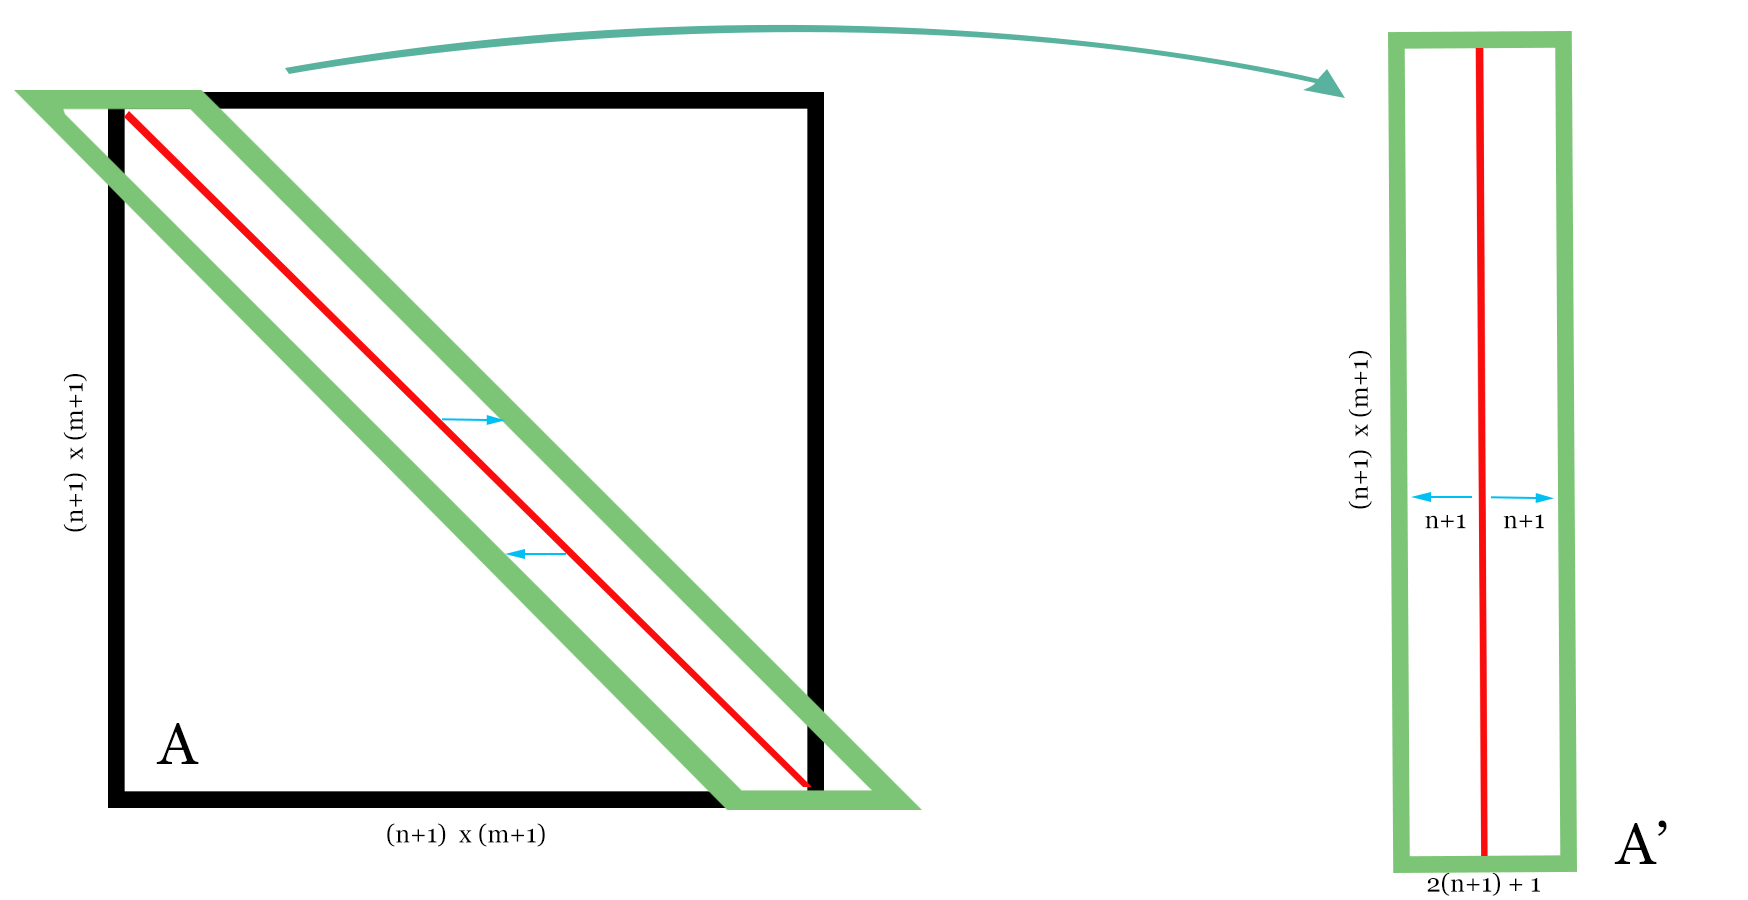
\includegraphics[scale=1]{./img/matriz_A_idea.png}
		\vspace{1pt}
		\footnotesize\textit{Aquí se puede observar la matriz A completa y la A' siendo la banda. Nótese que tanto al final como al principio de A' hay elementos que no pertenecen a la matriz cuadrada.}
	\end{center}
	
	
Ya que la idea es tomar toda la banda como una matriz, esta va a tener la particularidad de que entre dos filas consecutivas habrá una columna de diferencia en la matriz cuadrada. Por ejemplo, tomemos dos filas consecutivas $f_1$ y $f_2$ en las que sus $2n+1$ elementos existan en la matriz cuadrada. Lo que se puede destacar es que los elementos $f_1[0]$ y $f_2[0]$ en la matriz cuadrada \textit{no estarán en la misma columna}, ya que representan a alementos de la banda y la misma está inclinada diagonalmente. Mirando la matriz con las filas aumentando hacia abajo, si asumimos que $f_1$ está arriba de $f_2$, luego en nuestro modelo $f_2$ estará corrida de una fila hacia abajo y una columna hacia la derecha en la matriz cuadrada. Si tomara otra fila $f_3$, la fila consecutiva abajo de $f_2$, sabemos que entre $f_2$ y $f_3$ los elementos en la misma columna en la nueva matriz estarán corridos una columna hacia la derecha en la matriz cuadrada, y además entre $f_1$ y $f_3$ habrá \textit{dos} columnas de diferencia. He aquí un dibujo que ilustra la situación:


	\begin{center}
		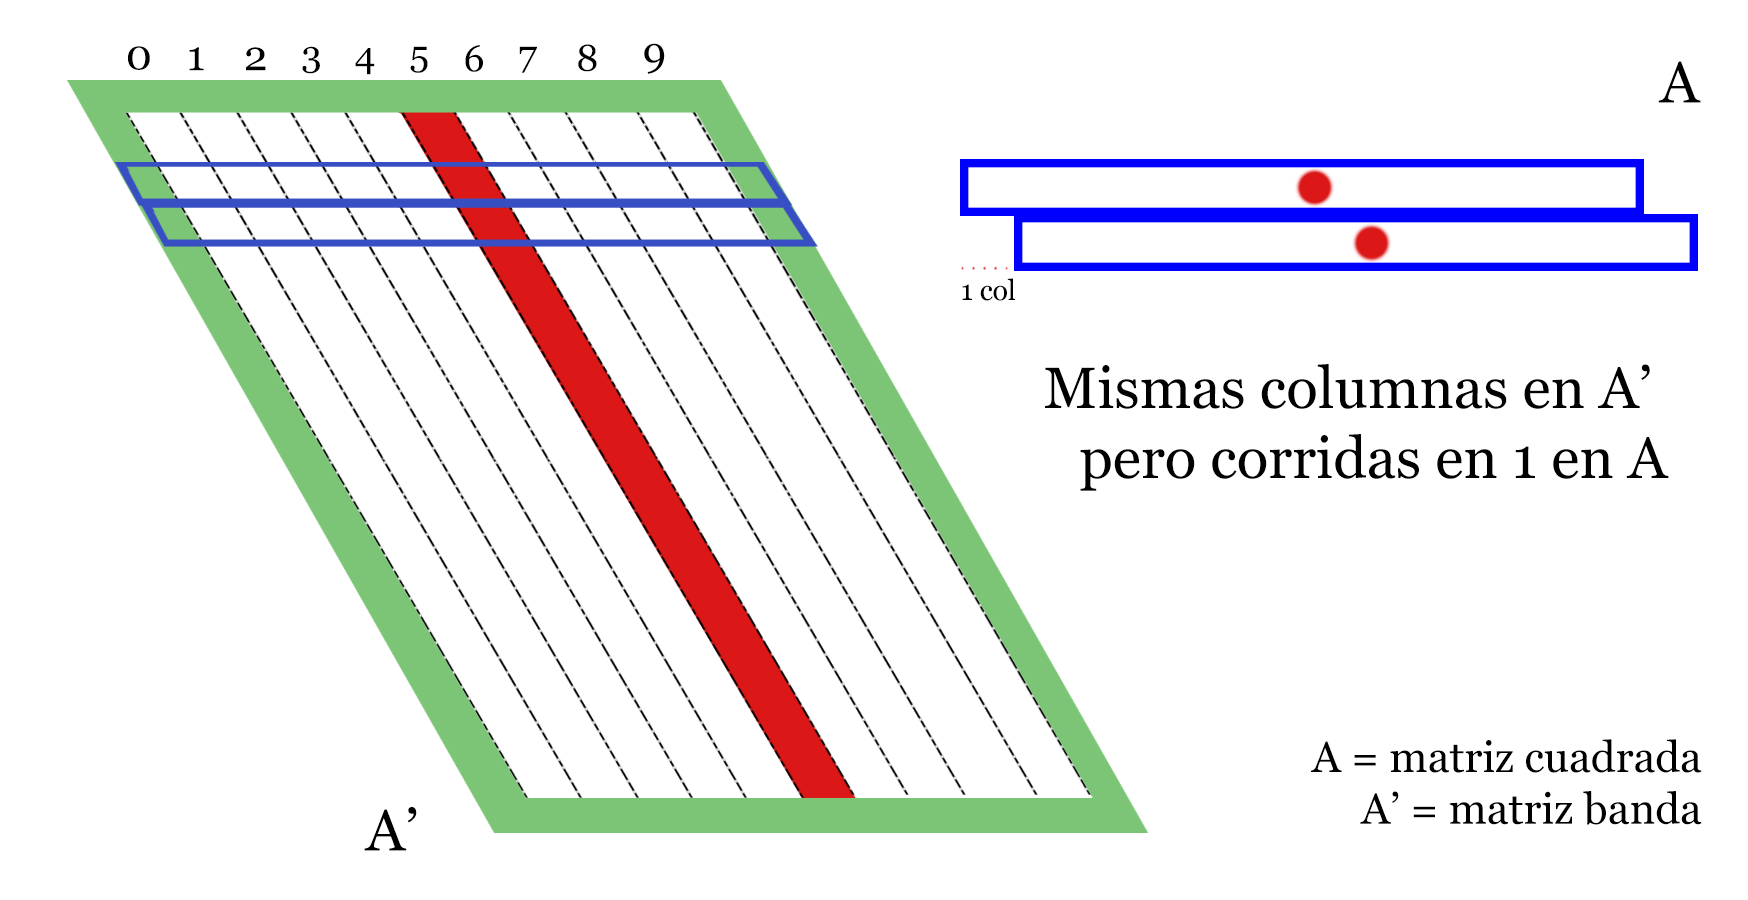
\includegraphics[scale=1]{./img/matriz_A_offset.png}
		\vspace{1pt}
		\footnotesize\textit{Aquí se puede apreciar el offset real respecto a las columnas que existe entre 1 o más filas en la matriz banda A'.}
	\end{center}
	
\vspace{\baselineskip}

\vspace{\baselineskip}
\par

Con esa estructura en mente, pasamos a ver las ideas para las modificaciones de la \textit{eliminación gaussiana} y la \textit{backward substitution}. Básicamente, al aplicar \textit{eliminación gaussiana}, queremos obtener la matriz que representa a \textbf{la banda de la matriz cuadrada después de haberla triangulado}. Esto quiere decir que \textit{no queremos triangular la nueva matriz $A$}, sino obtener los mismos resultados de la banda en la matriz cuadrada después de triangularla. Para ello debemos lograr una correspondencia de índices que nos permita utilizar sin problemas la nueva estructura, simulando que tenemos la completa con todos los demás 0 fuera de la banda.

Lo mismo sucede con la \textit{backward substitution}: si encontramos una correspondencia entre los índices de la matriz banda y la cuadrada que logre el mismo efecto que la otra implementación pero usando solamente esa porción de cada fila perteneciente a la banda, entonces el problema está resuelto.

\vspace{\baselineskip}
Esta es entonces la idea principal atrás de este tipo de implementación. Como se puede intuir, la complejidad espacial para esta solución es menor que la otra, y veremos también que temporalmente esta implementación supera claramente a la otra (ya que se realizarían muchísimas menos iteraciones para la \textit{eliminación gaussiana} y para resolver la matriz triangular). En la sección de \textbf{Implementación} se verá entonces en detalle como se pone en marcha esta solución.

\subsection{Implementación}

\subsection{Experimentación}

	En esta sección utilizaremos distintos gráficos para detallar los experimentos realizados. 

	Utilizamos gráficos de temperatura para validar el funcionamiento de nuestro algoritmo heurístico de eliminación de sanguijuelas. A continuación vemos el resultado del algoritmo sin eliminación, y posteriormente, el resultado con ella.

	\begin{center}
		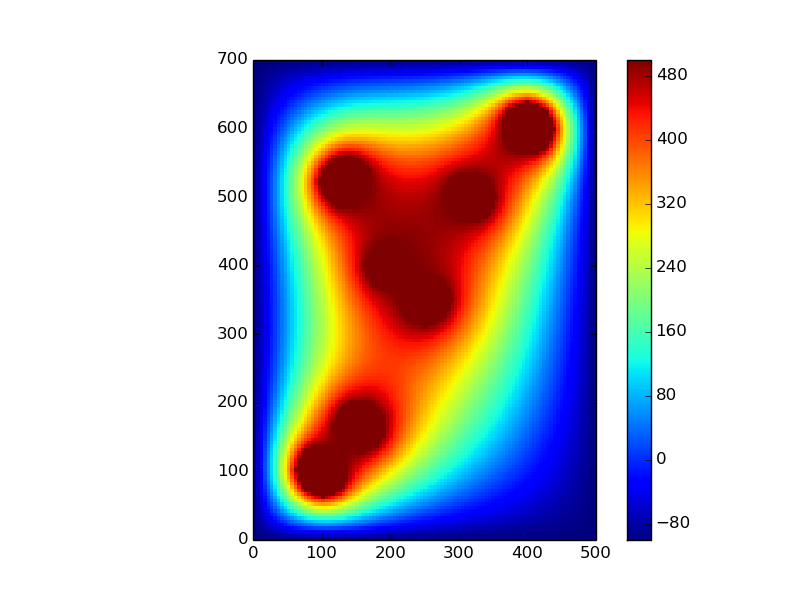
\includegraphics[scale=0.5]{./img/test5_sinkill.png}
	\end{center}

	\begin{center}
		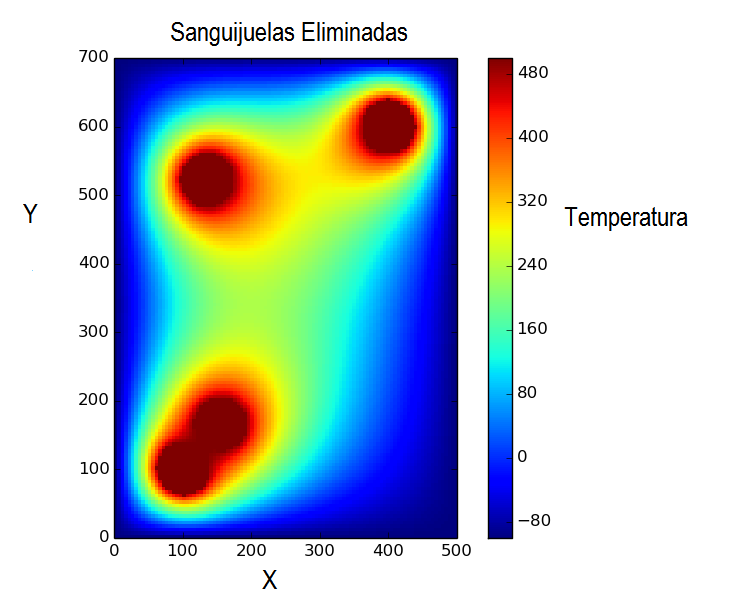
\includegraphics[scale=0.5]{./img/test5_conkill.png}
	\end{center}

	Como ya mencionamos, la heurística consta de eliminar las sanguijuelas más cercanas al centro del parabrisas hasta que el punto crítico sea menor al umbral. En este ejemplo, se eliminaron 3 sanguijuelas para lograr el objetivo.

	Este algoritmo posee como caso borde que las sanguijuelas se encuentren equidistantes con el centro del parabrisa. Los siguientes dos gráficos muestras el algoritmo sin y con eliminación respectivamente. La desición sobre qué sanguijuela eliminar es arbitraria y depende de cómo fue instanciado.

	\begin{center}
		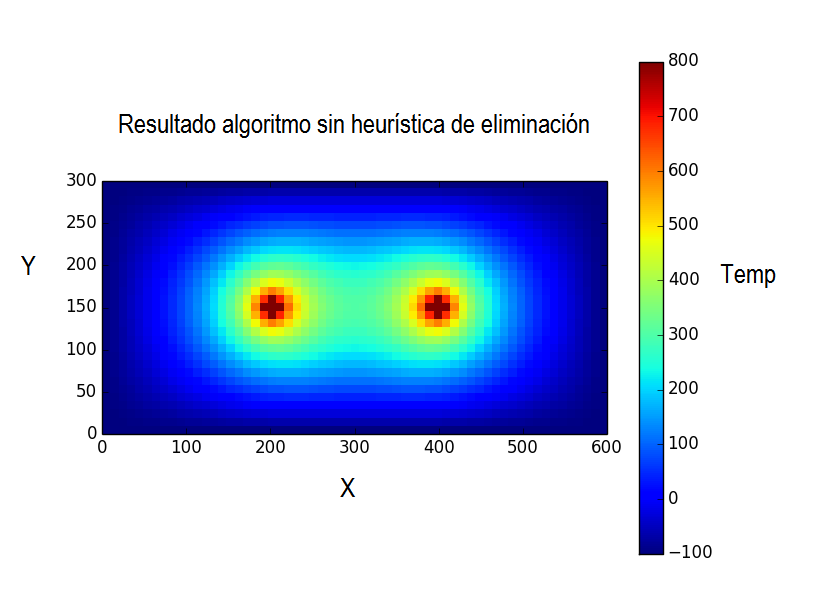
\includegraphics[scale=0.5]{./img/test6_sinkill.png}
	\end{center}

	\begin{center}
		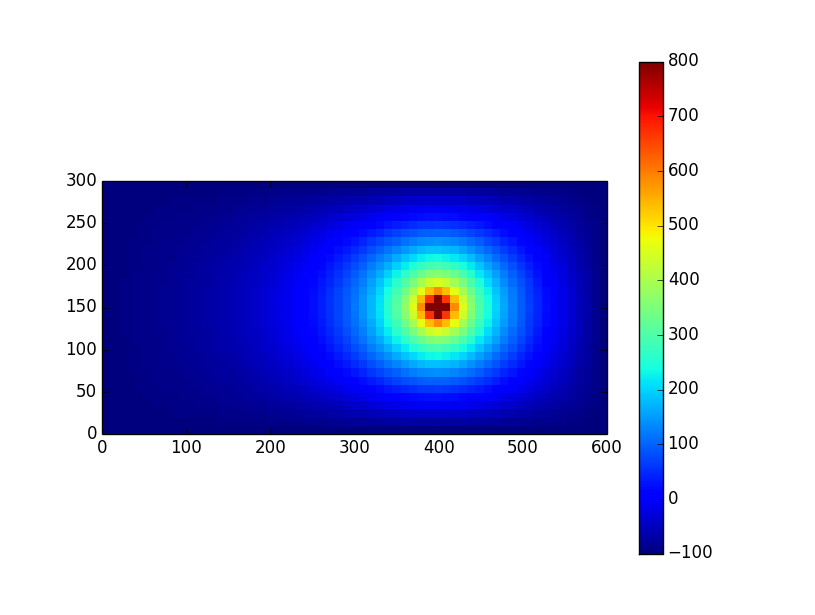
\includegraphics[scale=0.5]{./img/test6_conkill.png}
	\end{center}

	En nuestro caso, la sanguijuela izquierda fue eliminada.

	Cabe destacar que no siempre el resultado es el óptimo, es decir, no siempre se minimiza la cantidad de sanguijuelas removidas. Si tenemos un caso donde las sanguijuelas están equidistantes al centro del parabrisa, no se contabiliza en la desición de remoción la distancia al borde del parabrisa. El friod que emana de los bordes influye significativamente en el impacto que la sanguijuela tiene en el centro.

	Los tests anteriores poseen granularidad fija. Para vislumbrar cuál es el impacto de modificarla, utilizaremos nuevamente gráficos de temperatura. En todos los gráficos fijamos el tamaño del parabrisa (400 metros por 400 metros), la cantidad de sanguijuelas (una); y su temperatura (400 grados).

	\begin{center}
		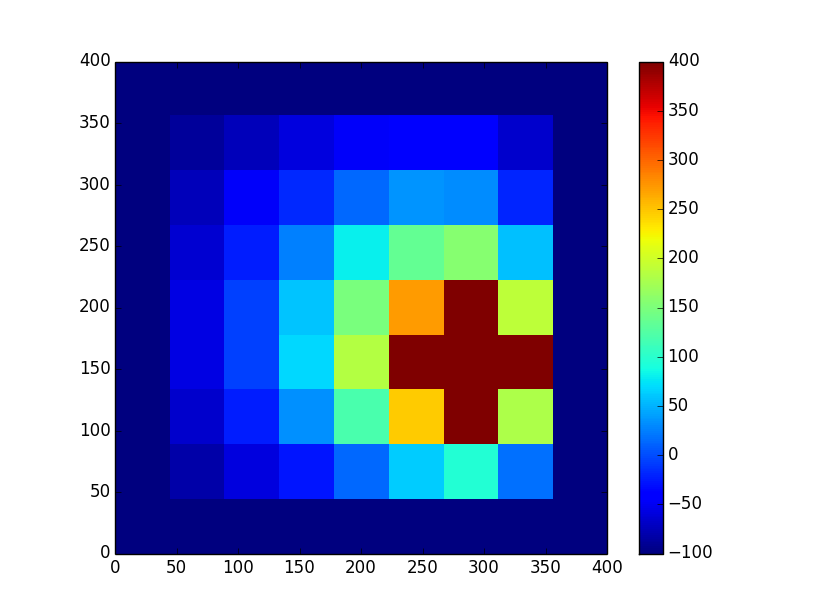
\includegraphics[scale=0.5]{./img/granularidad/g50_t400_sinkill.png}
	\end{center}

	El valor de temperatura en cada cuadrado de 50 x 50 es marcado, la diferencia entre bloques contiguos es muy alta. Es difícil distinguir a la sanguijuela ya que su forma no es circular.

	\begin{center}
		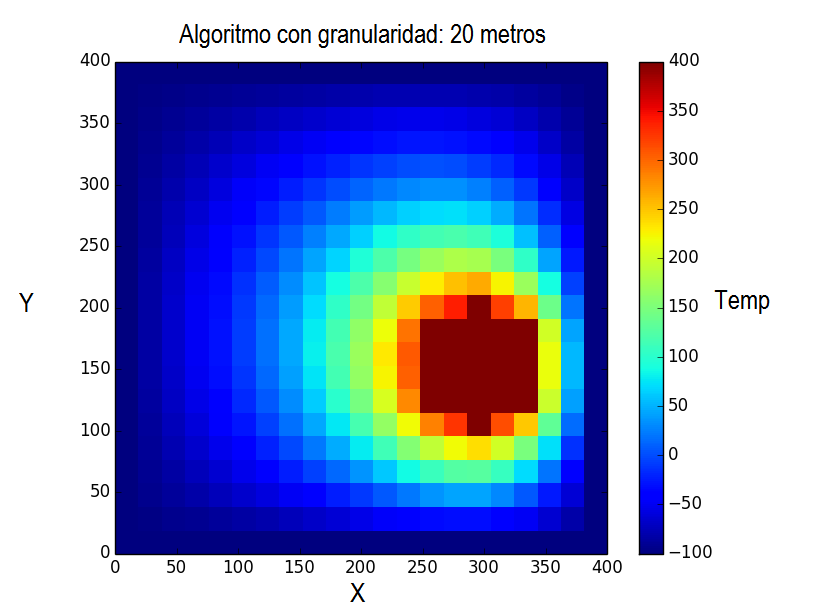
\includegraphics[scale=0.5]{./img/granularidad/g20_t400_sinkill.png}
	\end{center}

	La sanguijuela comienza a identificarse y se forman anillos con temperaturas decrecientes alrededor de ella. La distribución de la temperatura parece más homogénea.

	\begin{center}
		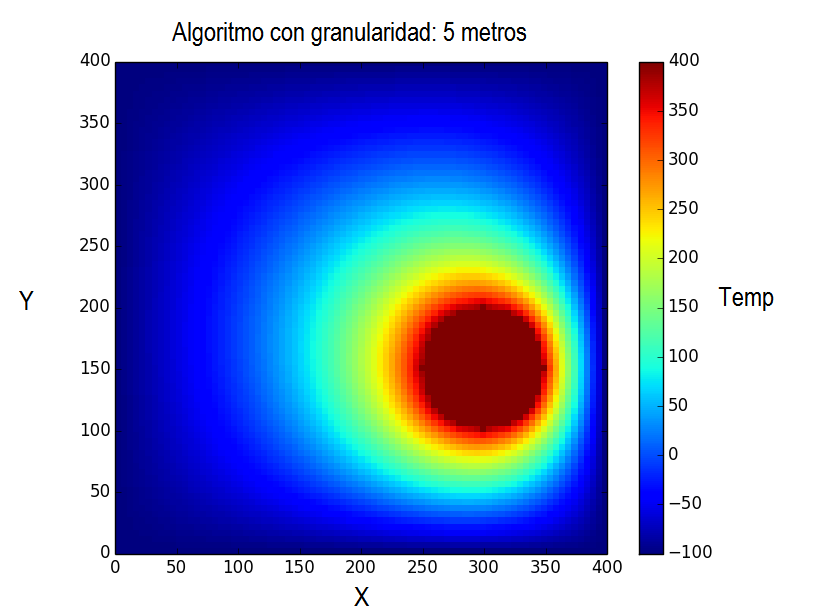
\includegraphics[scale=0.5]{./img/granularidad/g5_t400_sinkill.png}
	\end{center}

	El círculo de la sanguijuela ahora sí es completamente distinguible. Exceptuando los valores saturados, la temperatura a nivel global (y en el centro del parabrisas) parece aumentar. Esto puede deberse a que al tener una mayor granularidad, el algoritmo puede dispersar mejor el calor, ajustándose mejor a la realidad.

	\begin{center}
		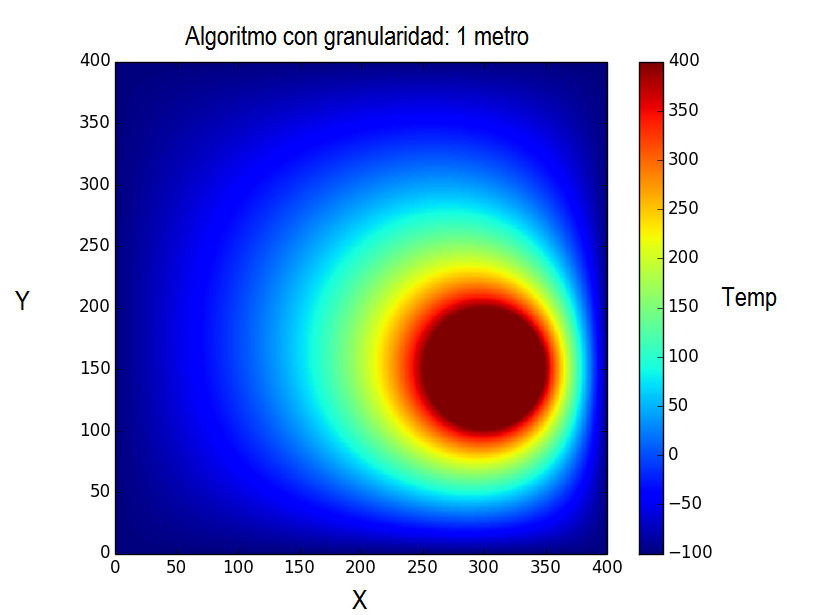
\includegraphics[scale=0.5]{./img/granularidad/g1_t400_sinkill.png}
	\end{center}

	La buena resolución de este gráfico permite tener una apreciación detallada sobre la dispersión de calor. Contribuye a la hipótesis: ``Cuanta más resolución, mejor dispersión de calor''. Sin embargo, como se verá posteriormente en este trabajo, existe una estrecha relación entre tiempo de cómputo y presición de los resultados. 
	
	Veamos entonces cómo cambia la temperatura en el punto central a medida que se modifica la granularidad.


	PONER GRAFICO DE TEMPERATURA EN PUNTO CENTRAL A MEDIDA QUE CAMBIA GRANULARIDAD
	PONER GRAFICO DE TEMPERATURA EN PUNTO CENTRAL A MEDIDA QUE CAMBIA GRANULARIDAD
	PONER GRAFICO DE TEMPERATURA EN PUNTO CENTRAL A MEDIDA QUE CAMBIA GRANULARIDAD
	PONER GRAFICO DE TEMPERATURA EN PUNTO CENTRAL A MEDIDA QUE CAMBIA GRANULARIDAD
	PONER GRAFICO DE TEMPERATURA EN PUNTO CENTRAL A MEDIDA QUE CAMBIA GRANULARIDAD	PONER GRAFICO DE TEMPERATURA EN PUNTO CENTRAL A MEDIDA QUE CAMBIA GRANULARIDAD

\par 
	Como se mencionó con anterioridad, existe una estrecha relación entre tiempo de computo y presición de los resultados. Es por esto, que se tomó el tiempo de ejecución del algoritmo para todos los casos que se mencionaron previamente, es decir, para el parabrisas de 400 metros por 400 metros, con una sola sanguijuela que posee 400 grados como temperatura. El parámetro que fue variando fue la granularidad, de igual forma a la realizada en los gráficos de temperatura que se expusieron. Estos valores fueron 50, 30, 5 y 1. 
	\par 
	La hipótesis planteada es que mientras menor es la granularidad para un mismo parabrisas, el tiempo de cómputo aumenta con creces. Es por esto, que se planteó correr cien iteraciones del algoritmo de resolución, con la intención de disminuir los outliers, para estos valores de granularidad  y obtener luego un promedio de la suma total de los mismos. Sin embargo, esto fue posible solo para los parabrisas con granularidad 50 y 30, ya que para aquellas granularidades menores, la resolución de cien instancias del problema contabilizaron más de 4 horas de cómputo para la matriz sin optimizar, es decir, sin aprovechar el uso de la matriz banda.
	\par 
	Es por esto, que con el objetivo de obtener más mediciones, se disminuyó la cantidad de iteraciones de resolución, disminuyendo también la precisión del experimento. Primero se intentó con 50 corridas del algoritmo, pero para la implementación con optimizaciones también demoró varias horas. De la misma manera, se redujo la cantidad de iteraciones nuevamente a 20 y posteriormente a 5 para el algoritmo que aprovecha el uso de la matriz banda. A pesar de que el algoritmo también demoró en el orden de horas para terminar, la implementación sin optimización alguna no pudo terminar \textit{una sola} corrida del algoritmo luego de más de 4 horas. 
	\par 
	Es por esto que a continuación se presenta el gráfico de granularidad respecto del tiempo con ambas implementaciones para granularidad 50 y 20, y solo la que usa la matriz banda para granularidad 5 y 1.
	\par 
	\begin{center}
		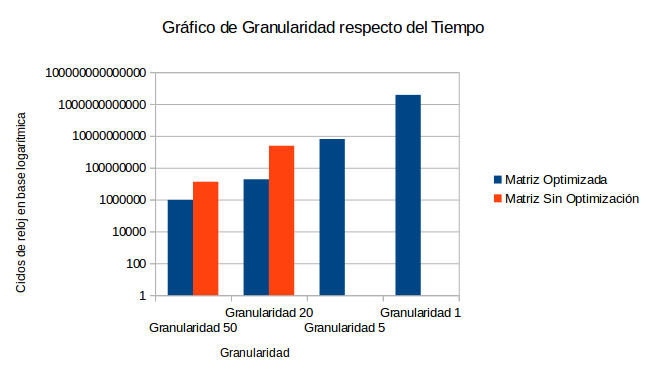
\includegraphics[scale=0.6]{./img/granularidad/granularidadrespectotiempo.png}
	\end{center}
	
	\par 
	Es necesario notar que el eje y, correspondiente a la cantidad de ciclos en promedio que demoró la resolución de las iteraciones, se encuentra en una escala logarítmica. 
	\par 
	Para ambos casos que se realizaron 100 iteraciones, es decir, para el test con granularidad 50 y el mismo con parámetro 20, la implementación que hace provecho de la matriz banda es extremadamente más rápida que aquella que no, sin siquiera tener en cuenta como disminuye la complejidad espacial. A su vez, se puede notar que a medida que disminuye la granularidad, la cantidad de ciclos por iteración del algoritmo aumenta al punto en el que no fue posible medirlo por restricciones temporales. 
	\par 
	De esta manera, la experimentación permite afirmar que la hipótesis respecto al aumento del tiempo respecto a la disminución de la granularidad es correcta y además queda explícito algo que damos por supuesto; la implementación que utiliza el hecho de ser matriz banda es mucho mejor a la implementación intuitiva de matriz, tanto espacial como temporalmente.
	
	\par 
	
	Por último, se realizaron experimentos para medir los tiempos del mismo test para el algoritmo que permite eliminar sanguijuelas y para aquel que no. 
	Debido a la implementación realizada, el algoritmo que puede eliminar sanguijuelas simplemente repite la implementación del mismo que no permite matar a las alimañas. Es por esto que es fácil de deducir que la versión optimizada es la que va a demorar menos tiempo. 
	\par 
	Para mostrar esto, se utilizó el test3 brindado por la cátedra. A continuación se mostrará el gráfico de temperatura correspondiente al mismo sin realizar la eliminación de sanguijuelas:
	
	\begin{center}
		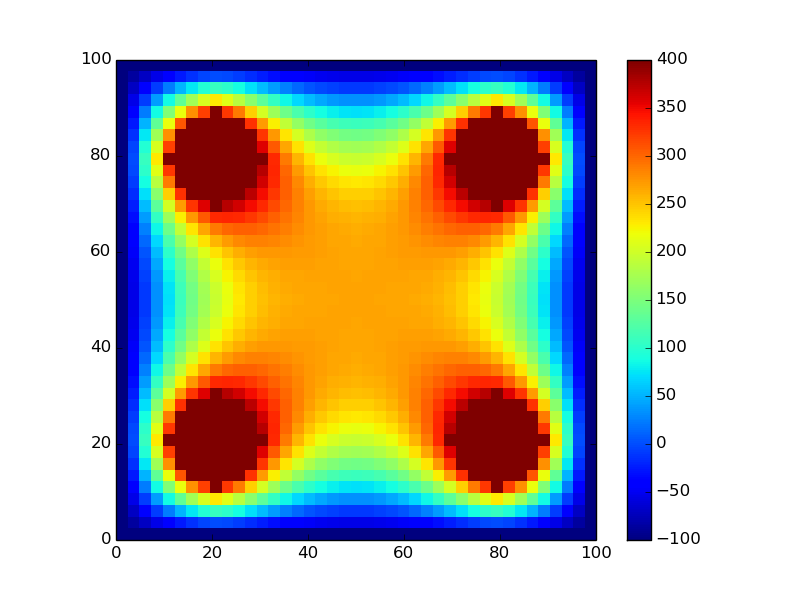
\includegraphics[scale=0.5]{./img/test3.png}
	\end{center}
	
	Ahora, el gráfico de temperatura del mismo test con la eliminación de sanguijuelas:
	
	\begin{center}
		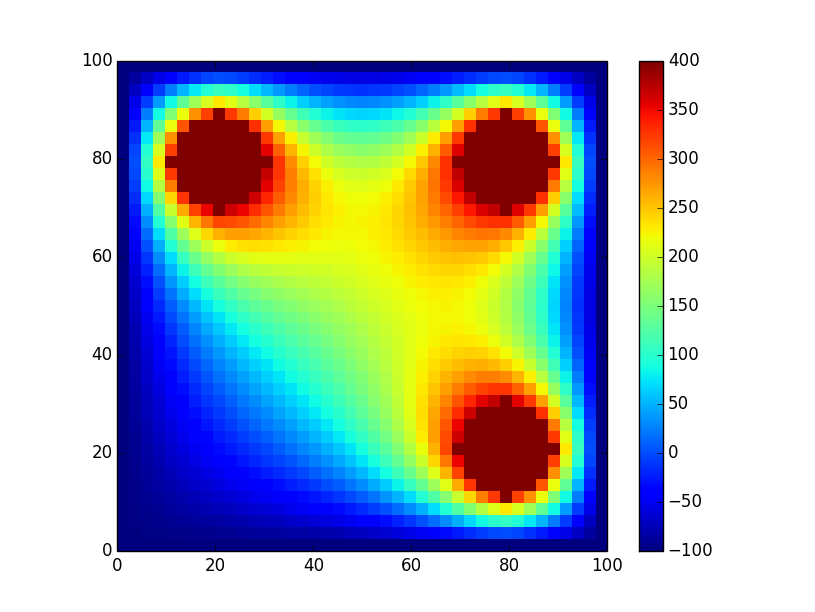
\includegraphics[scale=0.5]{./img/test3_con_kil.png}
	\end{center}
	
	\par 
	Como se puede ver, el algoritmo eliminó la sanguijuela ubicada en la parte inferior izquierda. Esto implica que la cantidad de veces que realizó dos veces el algoritmo(la primera vez para calcular el parabrisas obteniendo la imagen superior y posteriormente recalculando luego de eliminar una sanguijuela). 
	\par 
	A continuación, se presentará el gráfico de tiempos correspondiente al algoritmo con eliminación de sanguijuelas comparado con el que no:
\par 	
	\begin{center}
		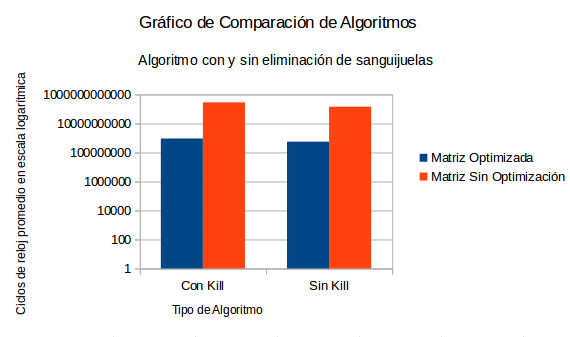
\includegraphics[scale=0.5]{./img/comparacionkill.png}
	\end{center}
	
	\par 
	Como se mencionó previamente, el algoritmo que hace uso de la matriz banda realiza el algoritmo en cualquiera de los dos modos (con eliminación de sanguijuelas o sin) más rápido que la otra implementación. 
	\par 
	Teniendo en cuenta que el eje y representa la cantidad de ciclos de reloj en promedio de 50 iteraciones, la diferencia de tiempos entre el algoritmo con eliminación y sin no parece tan grande. Sin embargo, al estar en una escala logarítmica, la diferencia es más pronunciada. Por ejemplo, en este caos, el promedio para el algoritmo optimizado sin eliminación es de 143135130237 ciclos de reloj en promedio, mientras que el mismo algoritmo pero matando sanguijuelas es 283591663824, el cual es aproximadamente el doble.
	
	\par 
	De esta manera, se ve que, como se dijo previamente, que el algoritmo con eliminación tarda más ciclos de reloj que el algoritmo que no se preocupa por la temperatura en el punto crítico. Además, se puede ver, tal como es esperado, que hay una relación entre cuántas sanguijuelas son eliminadas con el tiempo de ejecución del algoritmo. 
	
	
	
\section{Conclusión}

\section{Apéndice}

\section{Bibliografía y referencias} %arreglar cuando se termine 

\begin{itemize}
	\item \textbf{STL de C++}: \url{http://en.cppreference.com}.
	\par Para la función \texttt{rand()}, \url{http://en.cppreference.com/w/cpp/numeric/random/rand}.
	\par Para la función \texttt{sort()}, \url{http://en.cppreference.com/w/cpp/algorithm/sort}.
	\item Distribución de \texttt{rand()}?, \url{http://eternallyconfuzzled.com/arts/jsw\_art\_rand.aspx}
	\item \textbf{Contador de clocks}: \url{http://www.mcs.anl.gov/\~kazutomo/rdtsc.html}
\end{itemize}


\end{document}
